% Figure 4. Singularities of plane curves (printed page 36).
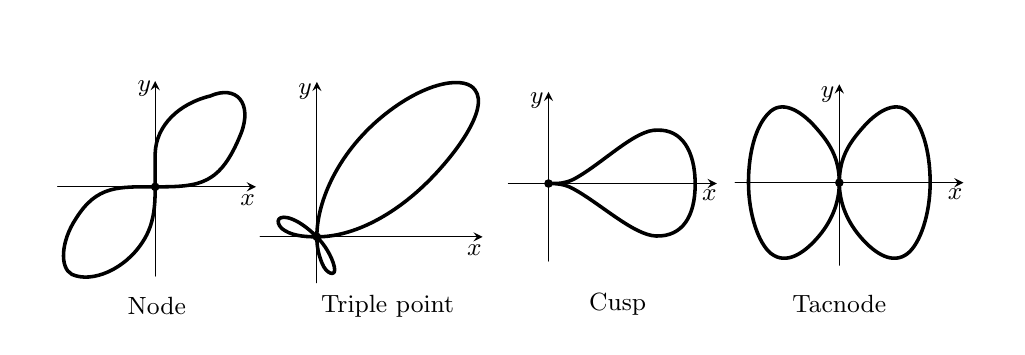
\begin{tikzpicture}[
    x=.3bp, y=-.3bp, line cap=round, line join=round, >=stealth,
    axis/.style={->,line width=.47bp},
    curve/.style={line width=1.28bp},
    every node/.style={inner sep=0pt,font=\small}
  ]
  \path[use as bounding box] (-24,-48) rectangle (1139.333,311.333);

  % At the node the two tangent lines are the coordinate axes.
  \coordinate (node) at (129,143);
  \draw[axis] (12,143) -- (250,143);
  \draw[axis] (129,250) -- (129,16);
  \draw[curve] (node)
    .. controls (183,143) and (207,141) .. (232,79)
    .. controls (246,43) and (227,20) .. (195,34)
    .. controls (158,43) and (130,69) .. (129,103)
    -- (node)
    .. controls (85,143) and (59,141) .. (34,181)
    .. controls (16,208) and (14,240) .. (29,248)
    .. controls (53,259) and (93,242) .. (114,209)
    .. controls (128,188) and (129,165) .. (node);
  \fill (node) circle[radius=1.55bp];
  \node at (116,25) {$y$};
  \node at (240,159) {$x$};
  \node at (131,286) {Node};

  % One lobe between each pair of adjacent tangents.
  \coordinate (triple) at (323,203);
  \draw[axis] (255,203) -- (522,203);
  \draw[axis] (323,258) -- (323,17);
  \draw[curve] (triple)
    .. controls (323,159) and (350,99) .. (406,55)
    .. controls (457,15) and (502,10) .. (513,27)
    .. controls (530,50) and (488,106) .. (454,139)
    .. controls (416,176) and (368,203) .. (triple);
  \draw[curve] (triple)
    .. controls (305,203) and (291,201) .. (281,193)
    .. controls (272,184) and (277,175) .. (294,182)
    .. controls (304,186) and (315,195) .. (triple)
    .. controls (332,212) and (341,226) .. (344,239)
    .. controls (347,252) and (334,248) .. (329,234)
    .. controls (325,224) and (323,215) .. (triple);
  \fill (triple) circle[radius=1.55bp];
  \node at (309,29) {$y$};
  \node at (512,219) {$x$};
  \node at (408,286) {Triple point};

  % The two halves of the cusp leave the origin along the positive x-axis.
  \coordinate (cusp) at (601,139);
  \draw[axis] (553,139) -- (803,139);
  \draw[axis] (601,232) -- (601,29);
  \draw[curve] (cusp)
    .. controls (615,139) and (620,139) .. (631,134)
    .. controls (665,116) and (706,73) .. (732,75)
    .. controls (761,74) and (777,100) .. (777,140)
    .. controls (777,178) and (762,203) .. (730,202)
    .. controls (703,201) and (662,162) .. (630,145)
    .. controls (621,140) and (612,139) .. (cusp);
  \fill (cusp) circle[radius=1.55bp];
  \node at (587,39) {$y$};
  \node at (794,153) {$x$};
  \node at (684,284) {Cusp};

  % The two lobes are both tangent to the vertical axis at the origin.
  \coordinate (tacnode) at (950,138);
  \draw[axis] (825,138) -- (1099,138);
  \draw[axis] (950,237) -- (950,20);
  \foreach \side in {-1,1} {
    \begin{scope}[shift={(tacnode)},xscale=\side]
      \draw[curve] (0,0)
        .. controls (0,-30) and (12,-48) .. (29,-67)
        .. controls (44,-84) and (66,-99) .. (82,-86)
        .. controls (99,-72) and (109,-39) .. (109,0)
        .. controls (109,38) and (97,73) .. (82,85)
        .. controls (64,99) and (43,85) .. (27,67)
        .. controls (10,48) and (0,25) .. (0,0);
    \end{scope}
  }
  \fill (tacnode) circle[radius=1.55bp];
  \node at (936,32) {$y$};
  \node at (1089,152) {$x$};
  \node at (950,284) {Tacnode};
\end{tikzpicture}
